\begin{figure}[ht]
\centering
% Thesis-wide categorical color palette
% Usage: % Thesis-wide categorical color palette
% Usage: % Thesis-wide categorical color palette
% Usage: \input{figures/palette} in any figure file
%
% Muted primary colors -- print-friendly, visually distinct.
% Inspired by Cooper Union's red/blue primaries, softened for
% academic figures. Use palA-palC for data series in scatter
% plots, line charts, bar charts, etc.

\definecolor{palA}{HTML}{1F77B4}   % Tableau blue
\definecolor{palB}{HTML}{D62728}   % Tableau red
\definecolor{palC}{HTML}{2CA02C}   % Tableau green
 in any figure file
%
% Muted primary colors -- print-friendly, visually distinct.
% Inspired by Cooper Union's red/blue primaries, softened for
% academic figures. Use palA-palC for data series in scatter
% plots, line charts, bar charts, etc.

\definecolor{palA}{HTML}{1F77B4}   % Tableau blue
\definecolor{palB}{HTML}{D62728}   % Tableau red
\definecolor{palC}{HTML}{2CA02C}   % Tableau green
 in any figure file
%
% Muted primary colors -- print-friendly, visually distinct.
% Inspired by Cooper Union's red/blue primaries, softened for
% academic figures. Use palA-palC for data series in scatter
% plots, line charts, bar charts, etc.

\definecolor{palA}{HTML}{1F77B4}   % Tableau blue
\definecolor{palB}{HTML}{D62728}   % Tableau red
\definecolor{palC}{HTML}{2CA02C}   % Tableau green


%% Panel (a): Stride 1
\begin{subfigure}[t]{0.45\textwidth}
\centering
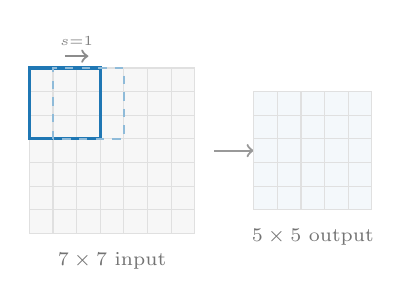
\begin{tikzpicture}[
    lbl/.style={font=\scriptsize, text=black!55},
]
\def\c{0.3}

% 7x7 input grid (empty)
\foreach \x in {0,...,6} {
    \foreach \y in {0,...,6} {
        \fill[gray!6, draw=black!12]
            (\x*\c, \y*\c) rectangle ++(\c, \c);
    }
}

% Kernel position 1 (solid blue, cols 0-2)
\draw[palA, very thick]
    (0, {4*\c}) rectangle ({3*\c}, {7*\c});

% Kernel position 2 (dashed, cols 1-3 -- one cell shift)
\draw[palA!50, thick, dashed]
    ({1*\c}, {4*\c}) rectangle ({4*\c}, {7*\c});

% Stride arrow above grid
\draw[->, thick, black!45]
    ({1.5*\c}, {7*\c + 0.15}) -- ({2.5*\c}, {7*\c + 0.15})
    node[midway, above, font=\tiny, text=black!50] {$s{=}1$};

% Input label
\node[lbl, anchor=north] at ({3.5*\c}, -0.12) {$7 \times 7$ input};

% Arrow to output
\draw[->, thick, black!40]
    ({7*\c + 0.25}, {3.5*\c}) -- ++(0.5, 0);

% 5x5 output grid
\def\ox{2.85}
\def\oy{0.3}
\foreach \x in {0,...,4} {
    \foreach \y in {0,...,4} {
        \fill[palA!5, draw=black!12]
            ({\ox + \x*\c}, {\oy + \y*\c})
            rectangle ++({\c}, {\c});
    }
}
\node[lbl, anchor=north] at ({\ox + 2.5*\c}, {\oy - 0.12})
    {$5 \times 5$ output};

\end{tikzpicture}
\subcaption{Stride $1$: the kernel shifts one cell per step.}
\label{fig:stride-one}
\end{subfigure}
\hfill
%% Panel (b): Stride 2
\begin{subfigure}[t]{0.45\textwidth}
\centering
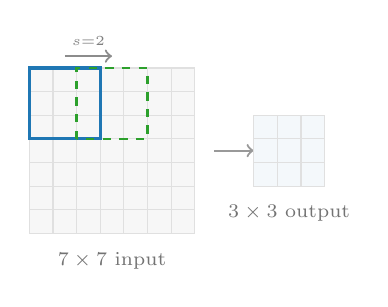
\begin{tikzpicture}[
    lbl/.style={font=\scriptsize, text=black!55},
]
\def\c{0.3}

% 7x7 input grid (empty)
\foreach \x in {0,...,6} {
    \foreach \y in {0,...,6} {
        \fill[gray!6, draw=black!12]
            (\x*\c, \y*\c) rectangle ++(\c, \c);
    }
}

% Kernel position 1 (solid blue, cols 0-2)
\draw[palA, very thick]
    (0, {4*\c}) rectangle ({3*\c}, {7*\c});

% Kernel position 2 (dashed green, cols 2-4 -- two cell shift)
\draw[palC, thick, dashed]
    ({2*\c}, {4*\c}) rectangle ({5*\c}, {7*\c});

% Stride arrow above grid
\draw[->, thick, black!45]
    ({1.5*\c}, {7*\c + 0.15}) -- ({3.5*\c}, {7*\c + 0.15})
    node[midway, above, font=\tiny, text=black!50] {$s{=}2$};

% Input label
\node[lbl, anchor=north] at ({3.5*\c}, -0.12) {$7 \times 7$ input};

% Arrow to output
\draw[->, thick, black!40]
    ({7*\c + 0.25}, {3.5*\c}) -- ++(0.5, 0);

% 3x3 output grid (smaller than panel a)
\def\ox{2.85}
\def\oy{0.6}
\foreach \x in {0,...,2} {
    \foreach \y in {0,...,2} {
        \fill[palA!5, draw=black!12]
            ({\ox + \x*\c}, {\oy + \y*\c})
            rectangle ++({\c}, {\c});
    }
}
\node[lbl, anchor=north] at ({\ox + 1.5*\c}, {\oy - 0.12})
    {$3 \times 3$ output};

\end{tikzpicture}
\subcaption{Stride $2$: the kernel shifts two cells per step.}
\label{fig:stride-two}
\end{subfigure}

\caption{Effect of stride on output size. Both panels use the same
  $7 \times 7$ input and $3 \times 3$ kernel. A larger stride means
  fewer kernel positions and a smaller output feature map.}
\label{fig:stride-effect}
\end{figure}
